% !TeX root = ../Thesis.tex

\chapter{An Approach to Agile Maneuvering}
\label{sec:approach-to-agile-maneuvering}

\section{Overview}

\section{System Dynamics}
\label{sec:system-dynamics}

\subsection{Choice of Reference Frames}
\begin{figure}[h!]
	\centering
	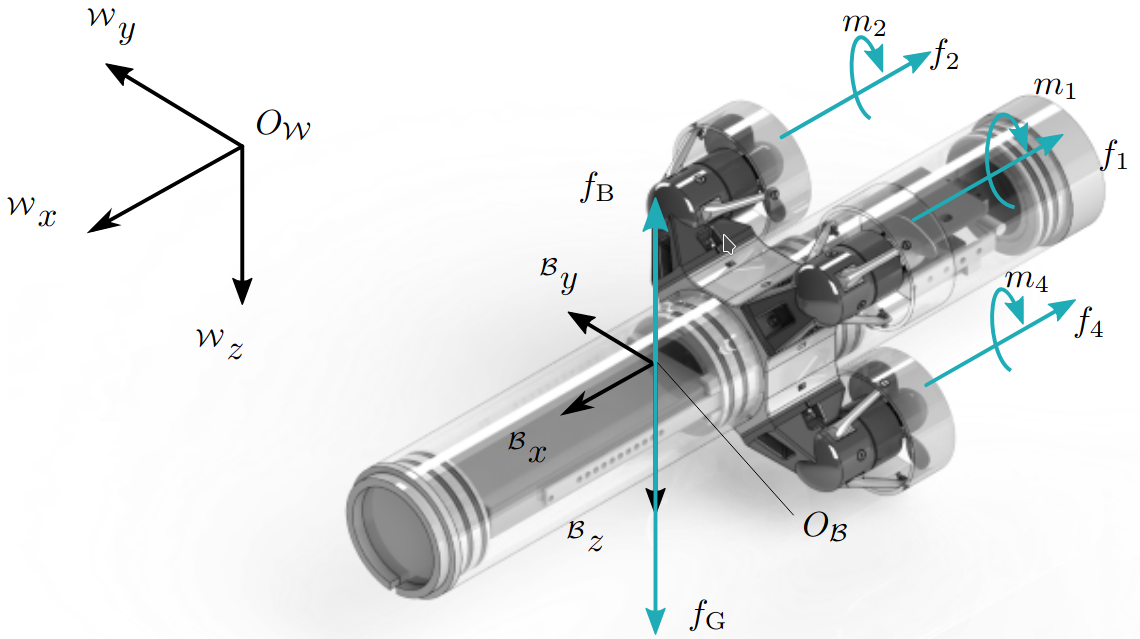
\includegraphics[width=0.7\linewidth]{placeholders/reference_frames.png}
	\caption{Definition of the world-fixed inertial frame of reference $\mathcal{W}$ and the body-fixed frame $\mathcal{B}$.}
\end{figure}
\subsubsection{World-fixed Frame}
\subsubsection{Body-fixed Frame}

\subsection{Equations of Motion}

The vector of absolute linear and angular velocities expressed in the body-fixed frame $\mathcal{B}$
\begin{equation}
	\nub = 
	\begin{bmatrix}
		\prescript{\mathcal{B}}{}{\vb} \\
		\prescript{\mathcal{B}}{}{\omeb}
	\end{bmatrix}
\end{equation}
with 
\begin{equation}
	\label{eq:velocities-in-body-frame}
	\prescript{\mathcal{B}}{}{\vb} = 
	\begin{bmatrix}
		u & v & w
	\end{bmatrix}^\top
	\text{ and }
	\prescript{\mathcal{B}}{}{\omeb} = 
	\begin{bmatrix}
		p & q & r
	\end{bmatrix}^\top
\end{equation}

Forces and moments with respect to the body-fixed frame.
\begin{equation}
	\taub = 
	\begin{bmatrix}
		\prescript{\mathcal{B}}{}{\fb} \\
		\prescript{\mathcal{B}}{}{\mb}
	\end{bmatrix}
\end{equation}
with 
\begin{equation}
	\prescript{\mathcal{B}}{}{\fb} = 
	\begin{bmatrix}
		X & Y & Z
	\end{bmatrix}^\top
	\text{ and }
	\prescript{\mathcal{B}}{}{\mb} = 
	\begin{bmatrix}
		K & M & N
	\end{bmatrix}^\top
\end{equation}

The vehicle's absolute pose $\etab$, i.e. position and orientation, expressed in $\mathcal{W}$, is
\begin{equation}
	\etab = 
	\begin{bmatrix}
		\prescript{\mathcal{W}}{}{\pbo} \\
		\prescript{\mathcal{W}}{}{\Theb_{\mathcal{W}\mathcal{B}}}
	\end{bmatrix}
\end{equation}
with
\begin{equation}
	\prescript{\mathcal{W}}{}{\pbo} = 
	\begin{bmatrix}
		x & y & z
	\end{bmatrix}^\top
	\text{ and }
	\Theb_{\mathcal{W}\mathcal{B}} =
	\begin{bmatrix}
		\phi & \theta & \psi
	\end{bmatrix}^\top,
\end{equation}
where $\prescript{\mathcal{W}}{}{\pbo}$ is the vehicle's position, i.e. the position of body frame origin $O_\mathcal{B}$, with respect to the world frame origin $O_\mathcal{W}$, and $\Theb_{\mathcal{W}\mathcal{B}}$ denotes the euler angle vector describing the transformation between $\mathcal{W}$ and $\mathcal{B}$ following the extrinsic $x$-$y$-$z$ convention.

We write the relation between the linear and angular velocities $\vlinbody$ and $\vangbody$ expressed in the body-fixed frame and the corresponding velocities in the world-fixed frame as
\begin{equation}
	\begin{bmatrix}
		\vlinworld \\
		\vangworld
	\end{bmatrix}
	=
	\underbrace{
	\begin{bmatrix}
		\Rbodyworld & \bm{0}_{3 \times 3} \\
		\bm{0}_{3 \times 3} & \TbodyWorld
	\end{bmatrix}
	}_{\scriptsize\coloneqq \Jb_\Theta}
	\begin{bmatrix}
		\vlinbody \\
		\vangbody
	\end{bmatrix},
\end{equation}
with is the rotation matrix 
\begin{equation}
	\label{eq:rotation-matrix}
	\Rbodyworld = 
	\begin{bmatrix}
		\text{c}\psi\text{c}\theta
		& \text{c}\psi \text{s}\theta \text{s}\phi - \text{s}\psi \text{c}\phi
		& \text{s}\psi \text{s}\phi + \text{c}\psi \text{c}\phi \text{s} \theta \\
		\text{s}\psi \text{c}\theta
		& \text{c}\psi \text{c}\phi + \text{s}\phi \text{s}\theta \text{s}\psi
		& \text{s}\theta \text{s}\psi \text{c}\phi - \text{c}\psi \text{s}\phi \\
		-\text{s}\theta
		& \text{c}\theta \text{s}\phi
		& \text{c}\theta \text{c}\phi
	\end{bmatrix}
\end{equation}
and the transformation matrix
\begin{equation}
	\label{eq:transformation}
	\TbodyWorld = 
	\begin{bmatrix}
		1 & \text{s}\phi \text{t}\theta & \text{c}\phi \text{t}\theta \\
		0 & \text{c}\phi & -\text{s}\phi \\
		0 & \frac{\text{s}\phi}{\text{t}\theta} & \frac{\text{c}\phi}{\text{c}\theta}
	\end{bmatrix},
\end{equation}
where $\text{s}\cdot$, $\text{c}\cdot$ and $\text{t}\cdot$ represent the functions $\sin(\cdot)$, $\cos(\cdot)$ and $\tan(\cdot)$, respectively.


\begin{equation}
	\label{eq:rigid-body-equation-of-motion}
	\Mrigid \nubp
	+ \Crigid(\nub) \nub
	= \taub
\end{equation}

\begin{equation}
	\label{eq:rigid-body-mass-matrix}
	\Mrigid =
	\begin{bmatrix}
		m \Ib_{3 \times 3} & \bm{0} \\
		\bm{0} & \Jb
	\end{bmatrix}
\end{equation}

Because \emph{principal axes of inertia} coincide with body frame axes, $\Jb$ will be diagonal, i.e. $\Jb = \text{diag}(J_x, J_y, J_z)$.

\begin{equation}
	\label{eq:6dof-equation-of-motion}
	\Mrigid \nubp + \Crigid(\nub) \nub +
	\underbrace{
		\Madded \nubp +
		\Cadded(\nub) \nub +
		\Dadded(\nub) \nub
	}_\text{hydrodynamic loads}
	+ 
	\underbrace{
		\gb(\etab)
	}_\text{\makebox[0pt]{hydrostatic load}}
	= \taub
\end{equation}
\todo{make sure to reference \cite{Fossen11}}
\begin{equation}
\Mb = \Mrigid + \Madded
\end{equation}
\todo[inline]{Replace \taub with $\inputbody$? Assumption of no other external loads?}

\begin{equation}
	\label{eq:input-vector}
	\inputbody =
	\begin{bmatrix}
		u_1 &
		0 &
		0 &
		u_2 &
		u_3 &
		u_4 
	\end{bmatrix}^\top
\end{equation}

\begin{equation}
	\Mbs = \left(m\Ib + \Mvadded\right), \text{ with }
	\Madded = \text{diag}\left(\Mvadded, \Jadded\right)
\end{equation}
\begin{equation}
	\Jbs = \left(\Jb + \Jadded\right), \text{ with }
	\Dadded = \text{diag}(\Dvadded, \Domegaadded)
\end{equation}
\begin{equation}
	\label{eq:equation-of-motion-translational}
	\Mbs \vlinbodydot = \vlinbody \times \Mbs \vangbody - \Dvadded \vlinbody - \gb(\etab) + u_1 \eb_1
\end{equation}\todo{Muss es nicht nur die obere Haelfte von $\gb$ sein? Muesste $\Mbs$ nicht vor $\vlinbody$ stehen?}
\begin{equation}
	\label{eq:equation-of-motion-rotational}
	\Jbs \vangbodydot =
	\vlinbody \times \Mbs \vangbody
	- \vangbody \times \Jbs \vangbody
	- \Domegaadded \vangbody
	- \gb(\etab)
	+ \begin{bmatrix}
		u_2 & u_3 & u_4	
	\end{bmatrix}^\top
\end{equation}

We make the following assumptions:
\begin{itemize}
	\item Symmetry with respect to $xz$, $yz$ and $xy$ planes.
	\item The center of gravity lies in the origin $O_\mathcal{B}$ of the body-fixed frame $\mathcal{B}$.
	\item The difference in the magnitudes of buoyancy force and gravitational force is zero, i.e. the vehicle is neutrally buoyant. Therefore, the restoring force is assumed to be zero.
	\item The center of buoyancy and the center of gravity coincide. The resulting restoring moment will be zero.
	\item The vehicle's velocity is relatively small.
	\item The motion of the vehicle is uncoupled.
	\item The principal axes of inertia coincide with the body-fixed frame axes.
\end{itemize}
Using body symmetry for $xz$, $yz$ and $xy$ planes \todo{Fossen 7.5.5}
\begin{equation}
	\Madded =
	\text{diag}\left(X_{\up}, Y_{\vp}, Z_{\wpo}, K_{\pp}, M_{\qp}, N_{\rp}\right)
\end{equation}

In general, 
\begin{equation}
	\Db(\nub) = -\text{diag}(X_\text{u}, Y_\text{v}, Z_\text{w}, K_\text{p}, M_\text{q}, N_\text{r})
\end{equation}
\todo{Nicht-linearen Teil lass ich direkt weg, weil der auch nicht mal simuliert wird.}


\begin{figure}[h!]
	\centering
	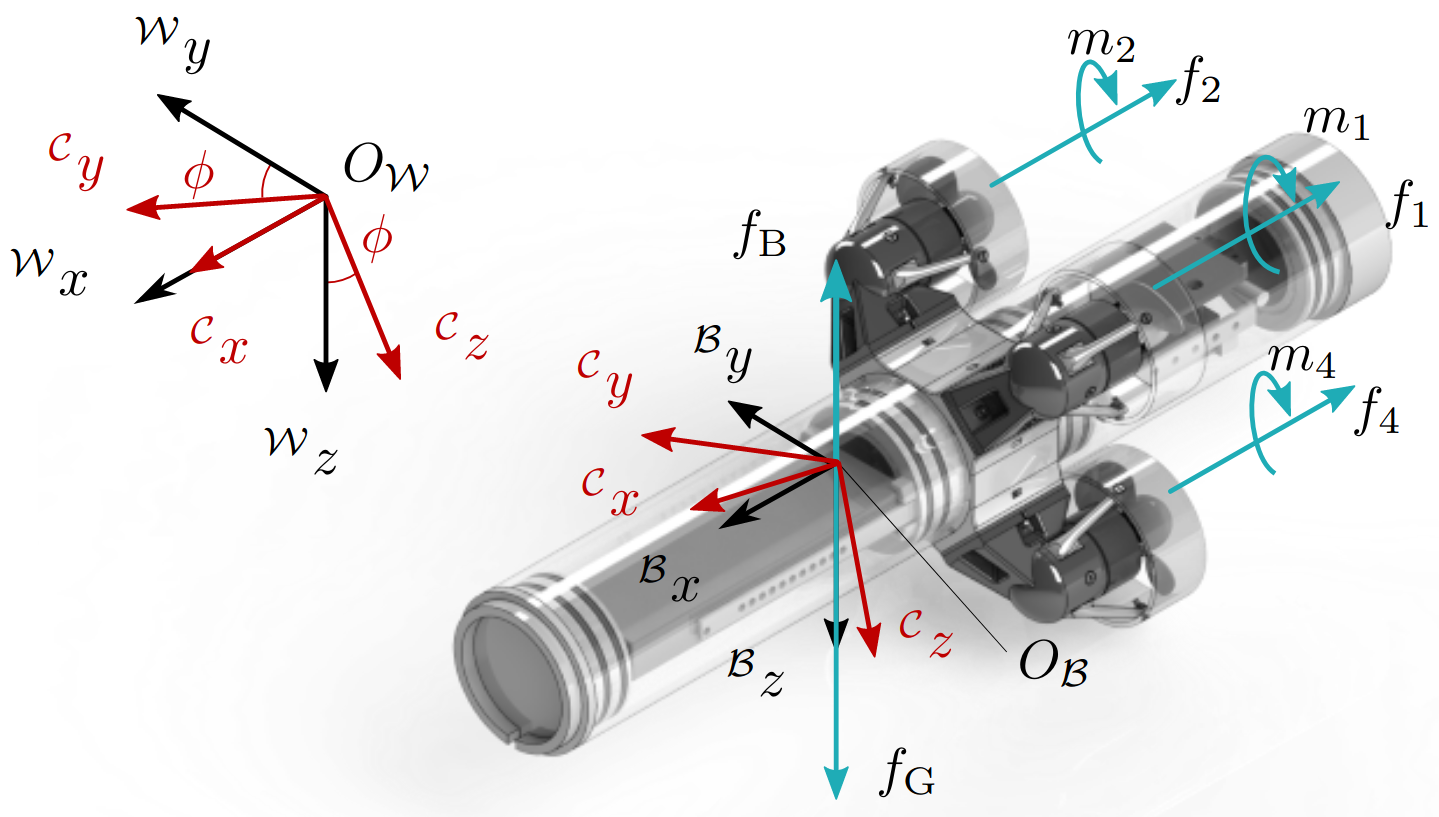
\includegraphics[width=0.7\linewidth]{placeholders/free_body.png}
	\caption{Free body diagram of the HippoCampus \mu AUV with buoyancy force $\bm{f}_\textrm{B}$, gravitational force $\bm{f}_\textrm{G}$, thruster forces $\bm{f}_\textrm{1:4}$, and thruster torques $\bm{m}_{1:4}$.}
\end{figure}
\begin{itemize}
	\color{red}
	\item Rigid body dynamics -> added hydrodynamic terms -> assumptions and simplifications -> yields simplified dynamic model
	\item Thruster model
	\begin{itemize}
		\item assume motor speed is reached instantaneously (fast in comparison to the body dynamics)
		\item assume quadratic thrust curve (Hastedt)
		\item neglect dead band
		\item neglect forward/reverse asymmetry.
	\end{itemize}
\end{itemize}

\subsection{Differential Flatness (Optional)}
{\color{red}
	show diff. flatness and motivate it by highlighting that it is useful for the trajectory-generation section
}

\section{Trajectory Generation}
\label{sec:trajectory-generation}

\begin{itemize}
	\color{red}
	\item make clear, that we do not care for any constrains (affine translational or input) for now. refer to the next section.
	\item Define the state variable consisting of translational variables and derivatives
\end{itemize}


\begin{equation}
	\label{eq:trajectory-state}
	\sbo = 
	\begin{bmatrix}
		\pbo \\ \vb \\ \ab	
	\end{bmatrix}
\end{equation}

\begin{equation}
	\label{eq:trajectory-state-per-axis}
	\sbo_{i} =
	\begin{bmatrix}
		p_{i} \\
		v_{i} \\
		a_{i}
	\end{bmatrix}
\end{equation}

\begin{equation}
	\label{eq:trajectory-state-derivative-per-axis}
	\sbp_\text{i} =
	\begin{bmatrix}
		v_{i} \\
		a_{i} \\
		j_{i}
	\end{bmatrix}
\end{equation}

\subsection{Kinematic Derivation of the jerk-optimal Trajectory}
\begin{itemize}
	\color{red}
	\item Define the cost function
	\item derive the minimum jerk solution per axis
	\item 
\end{itemize}

\begin{equation}
	\label{eq:cost-function}
	J_\text{\Sigma} = \frac{1}{T} \int_{0}^{T}\left\lVert \jb(t)\right\rVert^2 \text{d}t
\end{equation}

\begin{equation}
	\label{eq:cost-function-per-axis}
	J_\text{\Sigma} = \sum_{i=1}^{3}J_\text{i}, \text{ where } J_{i} = \frac{1}{T}\int_{0}^{T}j_i(t)^2\text{d}t
\end{equation}

\begin{equation}
	\label{eq:optimal-trajectory-per-axis}
	\sbo^* = 
	\begin{bmatrix}
		\frac{\alpha}{120}t^5
		+ \frac{\beta}{24}t^4
		+ \frac{\gamma}{6}t^3
		+ \frac{a_0}{2}t^2
		+ v_0 t
		+ p_0
		\\
		\frac{\alpha}{24} t^4
		+ \frac{\beta}{6} t^3
		+ \frac{\gamma}{2} t^2
		+ a_0 t
		+ v_0
		\\
		\frac{\alpha}{6} t^3
		+ \frac{\beta}{2} t^2
		+ \gamma t
		+ a_0
	\end{bmatrix}
\end{equation}

\begin{equation}
	\label{eq:trajectory-coefficients}
	\begin{bmatrix}
		\alpha \\
		\beta \\
		\gamma
	\end{bmatrix}
	=
	\begin{bmatrix}
		720 & -360T & 60T^2 \\
		-360T & 168T^2 * -24T^3 \\
		60T^2 & -24T^3 & 3T^4

	\end{bmatrix}
	\begin{bmatrix}
		\Delta p \\
		\Delta v \\
		\Delta a
	\end{bmatrix}
\end{equation}

\begin{equation}
	\label{eq:trajectory-delta-state}
	\begin{bmatrix}
		\Delta p \\
		\Delta v \\
		\Delta a
	\end{bmatrix}
	= 
	\begin{bmatrix}
		p_\text{f} - p_0 - v_0 T - \frac{1}{2}a_0 T^2 \\
		v_\text{f} - v_0 - a_0 T \\
		a_\text{f} - a_0
	\end{bmatrix}
\end{equation}


\subsection{Sampling Strategy}
\begin{itemize}
	\color{red}
	\item how to choose the final state to reach the high level goal, i.e. catching the ring as proposed scenario.
	\begin{itemize}
		\item vehicle tip position inside the ring
		\item different final attitudes possible (sampling on a section of a sphere around final tip position)
		\item calculate actual vehicle's position based on that
	\end{itemize}
	\item higher variety of final states increases chance to generate a feasible solution -> refer to following section
	\item introduce additional rotated inertial system to specify axis components or let them unspecified
	\item stress out the difference to MuellerHehn15, due to velocity dependency.
\end{itemize}
\begin{figure}[h!]
	\centering
	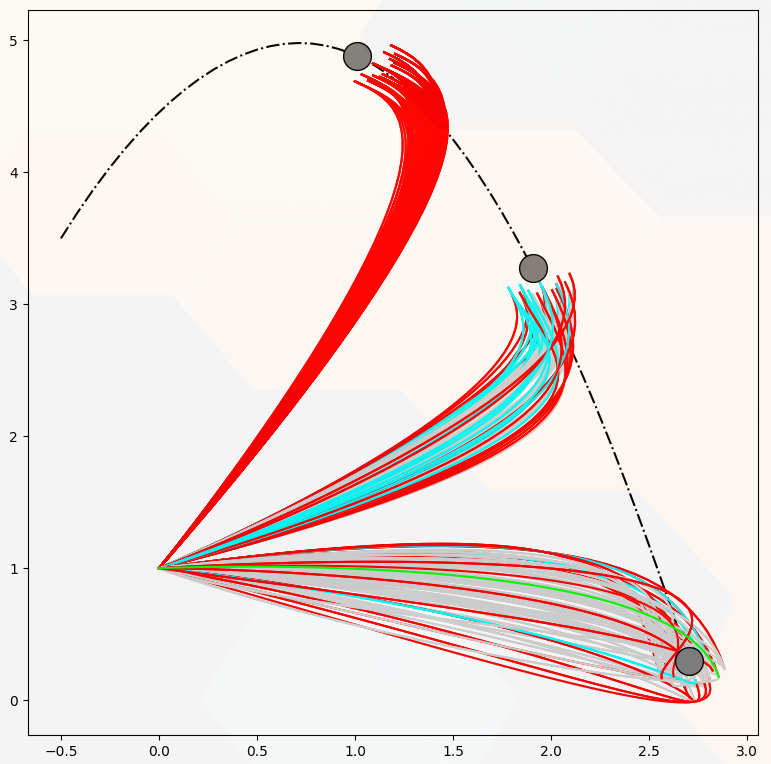
\includegraphics[width=0.7\linewidth]{placeholders/generation_example.png}
	\caption{Generated trajectories for different final states and time horizons.}
\end{figure}
\section{Feasibility of Trajectories}
\label{sec:feasibility}

\subsection{Input Feasibility}

\begin{equation}
	\label{eq:thrust-limits}
	\unit[0]{N} \leq f_\text{min} \leq f \leq f_\text{max}
\end{equation}

\begin{equation}
	\label{eq:body-rates-limit}
	\left\lVert\omeb\right\rVert
	\leq
	\omega_\text{max}
\end{equation}

\subsubsection{Thrust Input Feasibility}
\begin{itemize}
	\color{red}
	\item cubic instead of quadratic function is to be solved
	\item stress out, that feasibility criterium is quite coarse -> feasible solution might be classified as indeterminable
\end{itemize}

\begin{align}
	\label{eq:thrust-feasibility-equivilency-max}
	\max_{t \in \mathcal{T}} f(t)^2
	&\leq
	f_\text{max}^2 \\
	\label{eq:thrust-feasibility-equivilency-min}
	\min_{t \in \mathcal{T}} f(t)^2
	&\geq
	f_\text{min}^2
\end{align}

\subsubsection{Body Rates Input Feasibility}
\begin{itemize}
	\color{red}
	\item Insert dynamics into definition of jerk
\end{itemize}


\subsection{Position Feasibility}

\section{Obstacle/Collision Avoidance}
\begin{itemize}
	\color{red}
	\item Make clear, that obstacle avoidance is not built into the trajectory generation itself. 
	\item can be seen as subsequent feasibility check. 
\end{itemize}

\section{Control}
\label{sec:control}
\begin{itemize}
	\color{red}
	\item one could use the min jerk trajectory approach simply for generation -> feed-back control to keep the vehicle on track
	\item computational efficiency and real-time capability of approach enables trajectory generation to be used for implicit feedback. Regenerate trajectories in each control time step.
	\item body rates will change rather slowly compared to quadrocopters -> instead of using body rates as in MuellerHehn15, use target attitude and attitude control (actually the body rates are derived from a target attitude anyway)
\end{itemize}

\section{Implementation}
\label{sec:implementation}
